\documentclass[a4paper]{book}
\usepackage{makeidx}
\usepackage{natbib}
\usepackage{graphicx}
\usepackage{multicol}
\usepackage{float}
\usepackage{listings}
\usepackage{color}
\usepackage{ifthen}
\usepackage[table]{xcolor}
\usepackage{textcomp}
\usepackage{alltt}
\usepackage{ifpdf}
\ifpdf
\usepackage[pdftex,
            pagebackref=true,
            colorlinks=true,
            linkcolor=blue,
            unicode
           ]{hyperref}
\else
\usepackage[ps2pdf,
            pagebackref=true,
            colorlinks=true,
            linkcolor=blue,
            unicode
           ]{hyperref}
\usepackage{pspicture}
\fi
\usepackage[utf8]{inputenc}
\usepackage{mathptmx}
\usepackage[scaled=.90]{helvet}
\usepackage{courier}
\usepackage{sectsty}
\usepackage[titles]{tocloft}
\usepackage{doxygen}
\lstset{language=C++,inputencoding=utf8,basicstyle=\footnotesize,breaklines=true,breakatwhitespace=true,tabsize=8,numbers=left }
\makeindex
\setcounter{tocdepth}{3}
\renewcommand{\footrulewidth}{0.4pt}
\renewcommand{\familydefault}{\sfdefault}
\hfuzz=15pt
\setlength{\emergencystretch}{15pt}
\hbadness=750
\tolerance=750
\begin{document}
\hypersetup{pageanchor=false,citecolor=blue}
\begin{titlepage}
\vspace*{7cm}
\begin{center}
{\Large \-Reference \-Manual}\\
\vspace*{1cm}
{\large \-Generated by Doxygen 1.7.5.1}\\
\vspace*{0.5cm}
{\small Fri Nov 18 2011 19:04:42}\\
\end{center}
\end{titlepage}
\clearemptydoublepage
\pagenumbering{roman}
\tableofcontents
\clearemptydoublepage
\pagenumbering{arabic}
\hypersetup{pageanchor=true,citecolor=blue}
\chapter{\-Happy\-C\-M\-S \-Documentation}
\label{index}\hypertarget{index}{}\hypertarget{index_intro_sec}{}\section{\-Introduction}\label{index_intro_sec}
\-Happy \-C\-M\-S est un un outils entre un \-C\-M\-S est un framwork php \-M\-V\-C. \-Le but étant de développer avec la facilité d'un framwork mais que le résultat (notament la partie administration) soit intégré facilement dans une interface conventionnée. \-Il est basé sur le framework \-Cake\-P\-H\-P et conserve tous les conventions de \-Cake\-P\-H\-P. \-Il est principalement destiné aux développeurs (qui connaissent cake\-P\-H\-P de préférence). \-Après son installation vous pourrez continuer à développer votre application cake\-P\-H\-P comme d'habitude, et en plus de la gestion de certaines tache récurentes (utilisateurs, menus, pages simples..) vous aurez a disposition plusieurs controllers, models, et un behavior qui permette, en suivant un petit nombre de règles, d'intégré votre controller à \-Happy\-C\-M\-S. \par
\par
 \-Pour le moment le projet manque un peu d'unité, tout par un peu dans tout les sens, le temps de trouver des conventions. \-Pour le moment aussi le projet ne respect pas les convention cake\-P\-H\-P 2.\-0 ce qui est dommage. \par
\par
 \-Le projet étant encore à ses tout début, il est ouvert à toutes suggestions.\hypertarget{index_install_sec}{}\section{\-Installation}\label{index_install_sec}
\hypertarget{index_tools_subsec}{}\subsection{\-Tools required\-:}\label{index_tools_subsec}

\begin{DoxyItemize}
\item \-Cake\-P\-H\-P 1.\-3.$\ast$
\end{DoxyItemize}

\-Pour l'installation il suffit d'ajouter les fichiers de cake php à un projet vide connecté à la base de données (et dont le \-Security.\-salt a été correctement changé) et de lancer l'installation \-S\-I\-T\-E\-\_\-\-B\-A\-S\-E/install/ \par
\par
 \-L'installeur ajoute quelques tables et crée un utilisateurs admin.\hypertarget{index_example_sec}{}\section{\-Example}\label{index_example_sec}
\-Voici un exemple rapide pour offrir la possibilité à l'admin de rajouter des pages simples. \par
\-Un des principaux avantage de \-Happy\-C\-M\-S c'est qu'on a pas besoins de toucher à la base de données. \par
 \par
 \-Il nous faut un controller, un model, 2 vues et préciser à \-Happy\-C\-M\-S que notre extension offre une nouvelle possibilité. \par
\par
 \-On commence par crée une extension que l'on appel \char`\"{}pages\char`\"{}.\par
 config/extensions.\-php 
\begin{DoxyCode}
 Configure::write('Extensions.pages',array(
                                           'name'=>'Pages Simple',
                                           'views'=>array(
                                              'display'=>array(
                                                  'name'=>"Affichage d'une page
       simple"
                                                  )
                                          )));
\end{DoxyCode}
 \par
 \-Le code pour le controlleur change très peu d'un controlleur basique n'utilisant pas \-Happy\-C\-M\-S \par
\par
controllers/pages\-\_\-controller.\-php 
\begin{DoxyCode}
 class PagesController extends AppController
 {
                var $uses = array('Page');
                
                public function display($id)
                {
                        $this->set($this->Page->findById($id));
                }
                public function admin_display_edit($id)
                {
                        $this->request->data = $this->Page->findById($id);
                }

                public function admin_display_new($menu_id)
                {
                        //Le menu avec l'id = $menu_id veut afficher une
       nouvelle page
                        //Donc on crée cette page
                        $this->Page->create();
                        $this->Page->save(      array(
                                                        'Page'=>array(
                                                        'id'=>null,
                                                        'text'=>'Texte par
       défaut',
                                                        'published'=>1

                                                                )
                                                ));
                        //Ensuite on indique au menu l'argument qui devra être
       envoyé a la fonction display : l'id de la page

                        return $this->Page->id;
                }

 }
\end{DoxyCode}


\par
\-Pour le model il faut juste rajouter un \-Behavior \par
 \par
 models/page.\-php 
\begin{DoxyCode}
 class Page extends AppModel
 {
                var $actsAs = array('Content'=>array(
                                'extensionName'=>'pages'
                                                ));
                
 }
 *
\end{DoxyCode}
 \par
\-Pour la vue permettant l'édition d'une page, la différence réside dans l'utilisation d'un élément pour crée le formulaire. \par
\par
 views/pages/admin\-\_\-display\-\_\-edit.\-ctp 
\begin{DoxyCode}
 <?php
 echo $this->element('admin_create_form_item');
 echo $this->Form->input('text');
 echo $this->element('admin_end_form_item');
\end{DoxyCode}
 \par
\par
\-Pour la vue dislpay.\-ctp tout est permis.\hypertarget{index_copyright}{}\section{\-Copyright and License}\label{index_copyright}
\-G\-N\-U v3

\par
\par
 
\chapter{\-Class \-Index}
\section{\-Class \-Hierarchy}
\-This inheritance list is sorted roughly, but not completely, alphabetically\-:\begin{DoxyCompactList}
\item \contentsline{section}{\-App\-Controller}{\pageref{class_app_controller}}{}
\begin{DoxyCompactList}
\item \contentsline{section}{\-Categories\-Controller}{\pageref{class_categories_controller}}{}
\item \contentsline{section}{\-Configurations\-Controller}{\pageref{class_configurations_controller}}{}
\item \contentsline{section}{\-Contents\-Controller}{\pageref{class_contents_controller}}{}
\item \contentsline{section}{\-Extensions\-Controller}{\pageref{class_extensions_controller}}{}
\item \contentsline{section}{\-Files\-Controller}{\pageref{class_files_controller}}{}
\item \contentsline{section}{\-Links\-Controller}{\pageref{class_links_controller}}{}
\item \contentsline{section}{\-Menus\-Controller}{\pageref{class_menus_controller}}{}
\item \contentsline{section}{\-Pages\-Controller}{\pageref{class_pages_controller}}{}
\item \contentsline{section}{\-Users\-Controller}{\pageref{class_users_controller}}{}
\end{DoxyCompactList}
\item \contentsline{section}{\-Content}{\pageref{class_content}}{}
\item \contentsline{section}{\-Content\-Behavior}{\pageref{class_content_behavior}}{}
\item \contentsline{section}{\-Extension}{\pageref{class_extension}}{}
\item \contentsline{section}{\-Happy\-Route}{\pageref{class_happy_route}}{}
\item \contentsline{section}{\-Language}{\pageref{class_language}}{}
\item \contentsline{section}{\-Menu}{\pageref{class_menu}}{}
\item \contentsline{section}{\-User}{\pageref{class_user}}{}
\end{DoxyCompactList}

\chapter{\-Class \-Index}
\section{\-Class \-List}
\-Here are the classes, structs, unions and interfaces with brief descriptions\-:\begin{DoxyCompactList}
\item\contentsline{section}{\hyperlink{class_app_controller}{\-App\-Controller} }{\pageref{class_app_controller}}{}
\item\contentsline{section}{\hyperlink{class_categories_controller}{\-Categories\-Controller} }{\pageref{class_categories_controller}}{}
\item\contentsline{section}{\hyperlink{class_configurations_controller}{\-Configurations\-Controller} }{\pageref{class_configurations_controller}}{}
\item\contentsline{section}{\hyperlink{class_content}{\-Content} }{\pageref{class_content}}{}
\item\contentsline{section}{\hyperlink{class_content_behavior}{\-Content\-Behavior} }{\pageref{class_content_behavior}}{}
\item\contentsline{section}{\hyperlink{class_contents_controller}{\-Contents\-Controller} }{\pageref{class_contents_controller}}{}
\item\contentsline{section}{\hyperlink{class_extension}{\-Extension} }{\pageref{class_extension}}{}
\item\contentsline{section}{\hyperlink{class_extensions_controller}{\-Extensions\-Controller} }{\pageref{class_extensions_controller}}{}
\item\contentsline{section}{\hyperlink{class_files_controller}{\-Files\-Controller} }{\pageref{class_files_controller}}{}
\item\contentsline{section}{\hyperlink{class_happy_route}{\-Happy\-Route} }{\pageref{class_happy_route}}{}
\item\contentsline{section}{\hyperlink{class_language}{\-Language} }{\pageref{class_language}}{}
\item\contentsline{section}{\hyperlink{class_links_controller}{\-Links\-Controller} }{\pageref{class_links_controller}}{}
\item\contentsline{section}{\hyperlink{class_menu}{\-Menu} }{\pageref{class_menu}}{}
\item\contentsline{section}{\hyperlink{class_menus_controller}{\-Menus\-Controller} }{\pageref{class_menus_controller}}{}
\item\contentsline{section}{\hyperlink{class_pages_controller}{\-Pages\-Controller} }{\pageref{class_pages_controller}}{}
\item\contentsline{section}{\hyperlink{class_user}{\-User} }{\pageref{class_user}}{}
\item\contentsline{section}{\hyperlink{class_users_controller}{\-Users\-Controller} }{\pageref{class_users_controller}}{}
\end{DoxyCompactList}

\chapter{\-Class \-Documentation}
\hypertarget{class_app_controller}{
\section{\-App\-Controller \-Class \-Reference}
\label{class_app_controller}\index{\-App\-Controller@{\-App\-Controller}}
}
\-Inheritance diagram for \-App\-Controller\-:\begin{figure}[H]
\begin{center}
\leavevmode
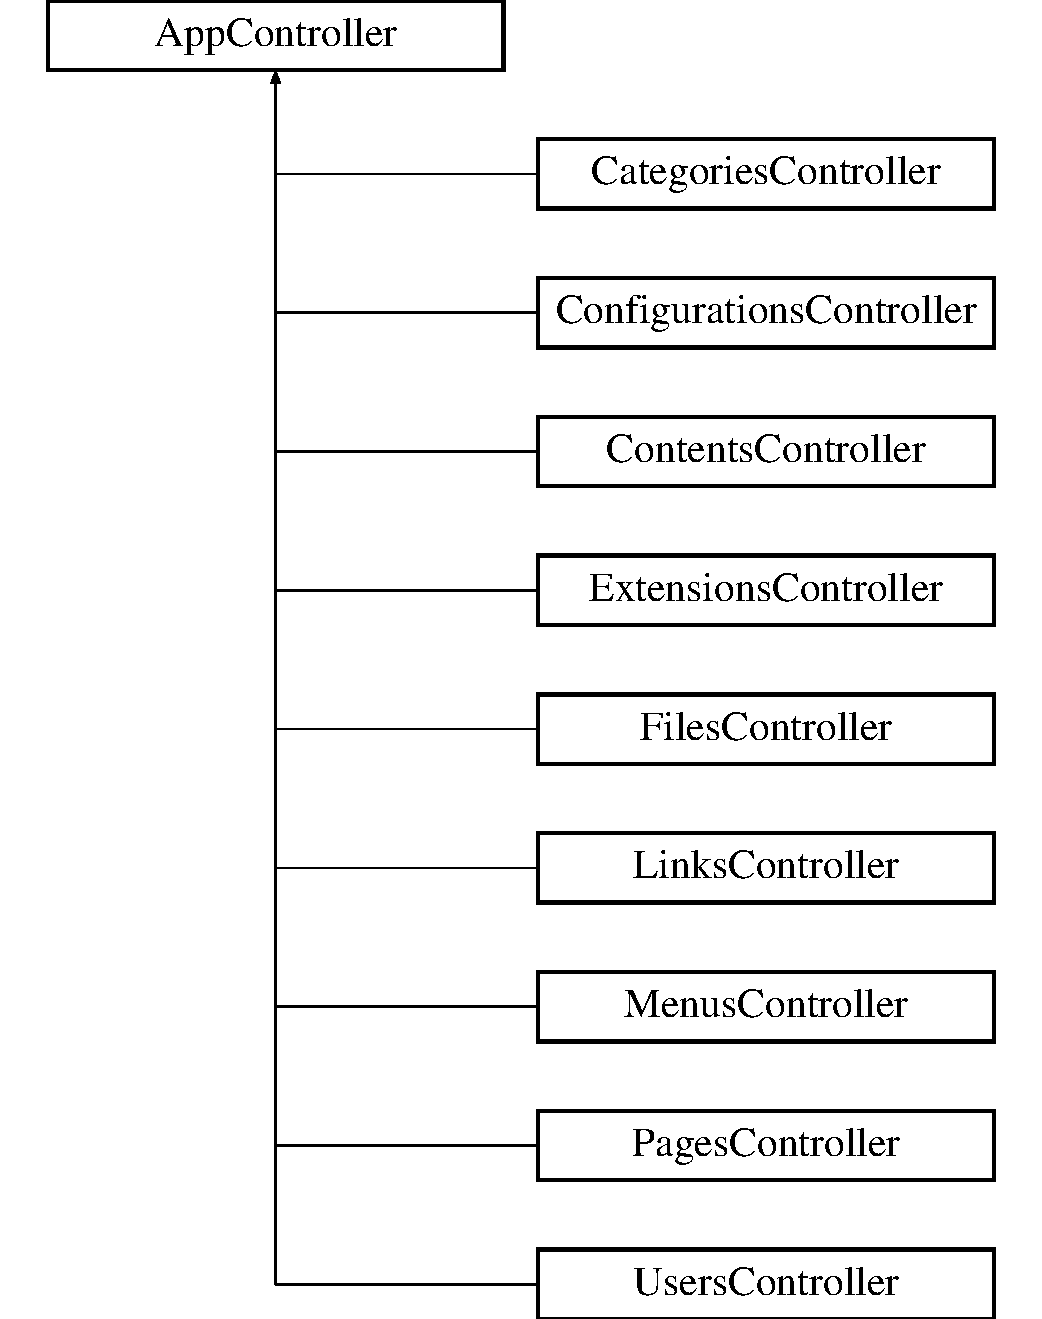
\includegraphics[height=10.000000cm]{class_app_controller}
\end{center}
\end{figure}
\subsection*{\-Public \-Member \-Functions}
\begin{DoxyCompactItemize}
\item 
\hyperlink{class_app_controller_ad883ad87afd78ad9a8f70416d1f9471e}{\-\_\-\-\_\-construct} ()
\item 
\hyperlink{class_app_controller_ae6932ff72664b2b2a7f0bffc3e7f9bc7}{before\-Filter} ()
\item 
\hypertarget{class_app_controller_ab11a05e10d035c3609fdb0efd218b6d4}{
{\bfseries check\-\_\-token} ()}
\label{class_app_controller_ab11a05e10d035c3609fdb0efd218b6d4}

\item 
\hypertarget{class_app_controller_a9c9b946429fb62af1c94bf31899f3395}{
{\bfseries admin\-\_\-save} ()}
\label{class_app_controller_a9c9b946429fb62af1c94bf31899f3395}

\item 
\hypertarget{class_app_controller_aa846b9844b6975d34d3f194f4b9ea14c}{
{\bfseries get\-Item} (\$id, \$assoc=true)}
\label{class_app_controller_aa846b9844b6975d34d3f194f4b9ea14c}

\item 
\hypertarget{class_app_controller_a6edf3d647292fb67a48e5f0e850353d5}{
{\bfseries get\-Items} (\$assoc=true, \$options=array())}
\label{class_app_controller_a6edf3d647292fb67a48e5f0e850353d5}

\item 
\hypertarget{class_app_controller_aea5a6426390bb3c855460962b5b6ef81}{
{\bfseries delete\-Item} (\$item\-\_\-id)}
\label{class_app_controller_aea5a6426390bb3c855460962b5b6ef81}

\item 
\hypertarget{class_app_controller_a4a98d0e4b2f49cf833a96cfb5fa981ed}{
{\bfseries get\-Views} (\$controller)}
\label{class_app_controller_a4a98d0e4b2f49cf833a96cfb5fa981ed}

\item 
\hypertarget{class_app_controller_a4c3fe84549c5925b54c0e290c9276064}{
{\bfseries admin\-\_\-to\-\_\-trash} (\$item\-\_\-id, \$lang=null)}
\label{class_app_controller_a4c3fe84549c5925b54c0e290c9276064}

\item 
\hypertarget{class_app_controller_a622c6741bfb65826af7bf42811d923af}{
{\bfseries admin\-\_\-to\-\_\-trash\-\_\-} (\$item\-\_\-id, \$lang=null)}
\label{class_app_controller_a622c6741bfb65826af7bf42811d923af}

\item 
\hypertarget{class_app_controller_aa09728c83a04669a8b36ad489babf466}{
{\bfseries admin\-\_\-params\-\_\-edit} ()}
\label{class_app_controller_aa09728c83a04669a8b36ad489babf466}

\end{DoxyCompactItemize}
\subsection*{\-Public \-Attributes}
\begin{DoxyCompactItemize}
\item 
\hypertarget{class_app_controller_a1649c9888b596557b60a06279beaf5fe}{
{\bfseries \$components} = array(\char`\"{}\-Auth\char`\"{},\char`\"{}\-Session\char`\"{})}
\label{class_app_controller_a1649c9888b596557b60a06279beaf5fe}

\item 
\hypertarget{class_app_controller_acdc4943ef51e546233a9fa724f4019ee}{
{\bfseries \$uses} = array()}
\label{class_app_controller_acdc4943ef51e546233a9fa724f4019ee}

\item 
\hypertarget{class_app_controller_a1d625be7647dafc4f218c2a320cab95b}{
{\bfseries \$helpers} = array('html','javascript','form',\char`\"{}\-Session\char`\"{},'\-Happy')}
\label{class_app_controller_a1d625be7647dafc4f218c2a320cab95b}

\item 
\hypertarget{class_app_controller_ae7d246eea37c34fa71ead8b36637bdf9}{
{\bfseries \$\-Hmodel\-\_\-name} = '\hyperlink{class_content}{\-Content}'}
\label{class_app_controller_ae7d246eea37c34fa71ead8b36637bdf9}

\item 
\hypertarget{class_app_controller_a9b4468e8b744c92dc2a128453c31349b}{
{\bfseries \$\-Hforce\-\_\-all\-\_\-languages} = false}
\label{class_app_controller_a9b4468e8b744c92dc2a128453c31349b}

\item 
\hypertarget{class_app_controller_ab189a47a78df5b8e4150b44adaa4e274}{
{\bfseries \$online} = false}
\label{class_app_controller_ab189a47a78df5b8e4150b44adaa4e274}

\item 
\hypertarget{class_app_controller_a429b64646f461eb735b402fdccd32202}{
{\bfseries \$\-\_\-requested\-Language} = null}
\label{class_app_controller_a429b64646f461eb735b402fdccd32202}

\end{DoxyCompactItemize}
\subsection*{\-Protected \-Member \-Functions}
\begin{DoxyCompactItemize}
\item 
\hypertarget{class_app_controller_a2e93f159461156d4c437ca3a4184aa03}{
{\bfseries unlink} (\$extension, \$file)}
\label{class_app_controller_a2e93f159461156d4c437ca3a4184aa03}

\item 
\hypertarget{class_app_controller_a2790fa5fed9d61809f0f8ea62d9cf4ad}{
{\bfseries get\-Extension\-Name} ()}
\label{class_app_controller_a2790fa5fed9d61809f0f8ea62d9cf4ad}

\item 
\hypertarget{class_app_controller_aa093c5a777af3a04528c31bf67721c37}{
{\bfseries save\-Item} (\$item)}
\label{class_app_controller_aa093c5a777af3a04528c31bf67721c37}

\item 
\hypertarget{class_app_controller_a480100d0f28cdd80eab1170dc52bb6d5}{
{\bfseries create\-Item} (\$params=null)}
\label{class_app_controller_a480100d0f28cdd80eab1170dc52bb6d5}

\end{DoxyCompactItemize}


\subsection{\-Constructor \& \-Destructor \-Documentation}
\hypertarget{class_app_controller_ad883ad87afd78ad9a8f70416d1f9471e}{
\index{\-App\-Controller@{\-App\-Controller}!\-\_\-\-\_\-construct@{\-\_\-\-\_\-construct}}
\index{\-\_\-\-\_\-construct@{\-\_\-\-\_\-construct}!AppController@{\-App\-Controller}}
\subsubsection[{\-\_\-\-\_\-construct}]{\setlength{\rightskip}{0pt plus 5cm}\-App\-Controller\-::\-\_\-\-\_\-construct (
\begin{DoxyParamCaption}
{}
\end{DoxyParamCaption}
)}}
\label{class_app_controller_ad883ad87afd78ad9a8f70416d1f9471e}
\-Constructor \-Hack for default model use 

\subsection{\-Member \-Function \-Documentation}
\hypertarget{class_app_controller_ae6932ff72664b2b2a7f0bffc3e7f9bc7}{
\index{\-App\-Controller@{\-App\-Controller}!before\-Filter@{before\-Filter}}
\index{before\-Filter@{before\-Filter}!AppController@{\-App\-Controller}}
\subsubsection[{before\-Filter}]{\setlength{\rightskip}{0pt plus 5cm}\-App\-Controller\-::before\-Filter (
\begin{DoxyParamCaption}
{}
\end{DoxyParamCaption}
)}}
\label{class_app_controller_ae6932ff72664b2b2a7f0bffc3e7f9bc7}
\-Token

\-Languages

\-Site \-Config

\-Auth

\-Layout \& menu

\hyperlink{class_extension}{\-Extension} \-Manager

load the extension info and params

\-The documentation for this class was generated from the following file\-:\begin{DoxyCompactItemize}
\item 
app\-\_\-controller.\-php\end{DoxyCompactItemize}

\hypertarget{class_categories_controller}{
\section{\-Categories\-Controller \-Class \-Reference}
\label{class_categories_controller}\index{\-Categories\-Controller@{\-Categories\-Controller}}
}
\-Inheritance diagram for \-Categories\-Controller\-:\begin{figure}[H]
\begin{center}
\leavevmode
\includegraphics[height=2.000000cm]{class_categories_controller}
\end{center}
\end{figure}
\subsection*{\-Public \-Member \-Functions}
\begin{DoxyCompactItemize}
\item 
\hypertarget{class_categories_controller_a062c83ecd4787750b390b9fcf09f8f9a}{
{\bfseries admin\-\_\-item\-\_\-edit} (\$item\-\_\-id)}
\label{class_categories_controller_a062c83ecd4787750b390b9fcf09f8f9a}

\item 
\hypertarget{class_categories_controller_aafda0171be86b56020be301149f0e9a8}{
{\bfseries admin\-\_\-threaded} (\$extension, \$lang)}
\label{class_categories_controller_aafda0171be86b56020be301149f0e9a8}

\item 
\hypertarget{class_categories_controller_ae1188eeb7e8e910273c617a801b6ea73}{
{\bfseries admin\-\_\-generate\-\_\-list} (\$extension)}
\label{class_categories_controller_ae1188eeb7e8e910273c617a801b6ea73}

\item 
\hypertarget{class_categories_controller_a3a0567c8e8506a75012dab09508dceec}{
{\bfseries admin\-\_\-to\-\_\-trash} (\$item\-\_\-id, \$extension)}
\label{class_categories_controller_a3a0567c8e8506a75012dab09508dceec}

\item 
\hypertarget{class_categories_controller_a9555daefb6b4915cda349afb03589471}{
{\bfseries admin\-\_\-save} ()}
\label{class_categories_controller_a9555daefb6b4915cda349afb03589471}

\item 
\hypertarget{class_categories_controller_ae1ed24d196ad30683bd3e5982cc53e00}{
{\bfseries get\-List} (\$extension)}
\label{class_categories_controller_ae1ed24d196ad30683bd3e5982cc53e00}

\end{DoxyCompactItemize}
\subsection*{\-Public \-Attributes}
\begin{DoxyCompactItemize}
\item 
\hypertarget{class_categories_controller_af0b01bb49dbdecdfd1d31a8605fa5067}{
{\bfseries \$uses} = array('\-Category')}
\label{class_categories_controller_af0b01bb49dbdecdfd1d31a8605fa5067}

\item 
\hypertarget{class_categories_controller_a2cbde1b8f51248c77d24484b2db3a436}{
{\bfseries \$\-Hforce\-\_\-all\-\_\-languages} = true}
\label{class_categories_controller_a2cbde1b8f51248c77d24484b2db3a436}

\end{DoxyCompactItemize}


\-The documentation for this class was generated from the following file\-:\begin{DoxyCompactItemize}
\item 
controllers/categories\-\_\-controller.\-php\end{DoxyCompactItemize}

\hypertarget{class_configurations_controller}{
\section{\-Configurations\-Controller \-Class \-Reference}
\label{class_configurations_controller}\index{\-Configurations\-Controller@{\-Configurations\-Controller}}
}
\-Inheritance diagram for \-Configurations\-Controller\-:\begin{figure}[H]
\begin{center}
\leavevmode
\includegraphics[height=2.000000cm]{class_configurations_controller}
\end{center}
\end{figure}
\subsection*{\-Public \-Member \-Functions}
\begin{DoxyCompactItemize}
\item 
\hypertarget{class_configurations_controller_afb65ad455f51060ef8a7b922cffca762}{
{\bfseries admin\-\_\-params\-\_\-edit} ()}
\label{class_configurations_controller_afb65ad455f51060ef8a7b922cffca762}

\item 
\hypertarget{class_configurations_controller_acc11d254295af530a6142b9f1d0f370a}{
{\bfseries get} ()}
\label{class_configurations_controller_acc11d254295af530a6142b9f1d0f370a}

\end{DoxyCompactItemize}
\subsection*{\-Public \-Attributes}
\begin{DoxyCompactItemize}
\item 
\hypertarget{class_configurations_controller_ab998262610b65039bd3c54de870c5b39}{
{\bfseries \$\-Hforce\-\_\-all\-\_\-languages} = true}
\label{class_configurations_controller_ab998262610b65039bd3c54de870c5b39}

\end{DoxyCompactItemize}


\-The documentation for this class was generated from the following file\-:\begin{DoxyCompactItemize}
\item 
controllers/configurations\-\_\-controller.\-php\end{DoxyCompactItemize}

\hypertarget{class_content}{
\section{\-Content \-Class \-Reference}
\label{class_content}\index{\-Content@{\-Content}}
}
\subsection*{\-Public \-Member \-Functions}
\begin{DoxyCompactItemize}
\item 
\hypertarget{class_content_a5aa30b5bfe817750c6a674a697e05b84}{
{\bfseries save} (\$data=\-N\-U\-L\-L, \$validate=true, \$field\-List=array())}
\label{class_content_a5aa30b5bfe817750c6a674a697e05b84}

\item 
\hyperlink{class_content_a7ee9747ba2041354415d3fda7b5d05aa}{save\-Item} (\$data=\-N\-U\-L\-L, \$validate=true, \$field\-List=array())
\item 
\hyperlink{class_content_ab3a13ad83d2423a47017b07ee0e31ae1}{item} (\$extension, \$item\-\_\-id, \$options=true)
\item 
\hyperlink{class_content_a513b15cf07c136d31c1699ba4d0733f2}{items} (\$extension, \$lang=null, \$assoc=true, \$options=array())
\item 
\hyperlink{class_content_a26aedd9db87f96b37874d9529d3841f7}{upload} (\$extension, \$lang, \$id, \$field, \$file)
\item 
\hypertarget{class_content_a9dd3b8e4c6db46fe56d213553dfc1242}{
{\bfseries filter\-Results} (\$results)}
\label{class_content_a9dd3b8e4c6db46fe56d213553dfc1242}

\end{DoxyCompactItemize}
\subsection*{\-Public \-Attributes}
\begin{DoxyCompactItemize}
\item 
\hypertarget{class_content_af8c3fc14dcbcb6b2f0a396761147e544}{
{\bfseries \$name} = \char`\"{}\-Content\char`\"{}}
\label{class_content_af8c3fc14dcbcb6b2f0a396761147e544}

\item 
\hypertarget{class_content_af06c60c5c6a0cd54ef35b449e744a460}{
{\bfseries \$display\-Field} = 'params'}
\label{class_content_af06c60c5c6a0cd54ef35b449e744a460}

\item 
{\bfseries \$belongs\-To}
\item 
\hypertarget{class_content_a0355358247e364f4a70ec19a6334d2f0}{
{\bfseries \$has\-And\-Belongs\-To\-Many} = array('\-Category')}
\label{class_content_a0355358247e364f4a70ec19a6334d2f0}

\end{DoxyCompactItemize}


\subsection{\-Member \-Function \-Documentation}
\hypertarget{class_content_ab3a13ad83d2423a47017b07ee0e31ae1}{
\index{\-Content@{\-Content}!item@{item}}
\index{item@{item}!Content@{\-Content}}
\subsubsection[{item}]{\setlength{\rightskip}{0pt plus 5cm}\-Content\-::item (
\begin{DoxyParamCaption}
\item[{\$}]{extension, }
\item[{\$}]{item\-\_\-id, }
\item[{\$}]{options = {\ttfamily true}}
\end{DoxyParamCaption}
)}}
\label{class_content_ab3a13ad83d2423a47017b07ee0e31ae1}
get an item witch belongs to the selected module.


\begin{DoxyParams}[1]{\-Parameters}
int & {\em \$module\-\_\-id} & the id of the module \\
\hline
int & {\em \$item\-\_\-id} & the id of the item \\
\hline
boolean & {\em \$assoc} & if true the result is an associated array \\
\hline
\end{DoxyParams}
\begin{DoxyReturn}{\-Returns}
\-The item 
\end{DoxyReturn}
\hypertarget{class_content_a513b15cf07c136d31c1699ba4d0733f2}{
\index{\-Content@{\-Content}!items@{items}}
\index{items@{items}!Content@{\-Content}}
\subsubsection[{items}]{\setlength{\rightskip}{0pt plus 5cm}\-Content\-::items (
\begin{DoxyParamCaption}
\item[{\$}]{extension, }
\item[{\$}]{lang = {\ttfamily null}, }
\item[{\$}]{assoc = {\ttfamily true}, }
\item[{\$}]{options = {\ttfamily array()}}
\end{DoxyParamCaption}
)}}
\label{class_content_a513b15cf07c136d31c1699ba4d0733f2}
get all items witch belongs to the selected module.


\begin{DoxyParams}[1]{\-Parameters}
int & {\em \$module\-\_\-id} & the id of the module \\
\hline
int & {\em \$item\-\_\-id} & the id of the item \\
\hline
boolean & {\em \$assoc} & if true the result is an associated array \\
\hline
\end{DoxyParams}
\begin{DoxyReturn}{\-Returns}
\-The items 
\end{DoxyReturn}
\hypertarget{class_content_a7ee9747ba2041354415d3fda7b5d05aa}{
\index{\-Content@{\-Content}!save\-Item@{save\-Item}}
\index{save\-Item@{save\-Item}!Content@{\-Content}}
\subsubsection[{save\-Item}]{\setlength{\rightskip}{0pt plus 5cm}\-Content\-::save\-Item (
\begin{DoxyParamCaption}
\item[{\$}]{data = {\ttfamily \-N\-U\-L\-L}, }
\item[{\$}]{validate = {\ttfamily true}, }
\item[{\$}]{field\-List = {\ttfamily array~(~)}}
\end{DoxyParamCaption}
)}}
\label{class_content_a7ee9747ba2041354415d3fda7b5d05aa}
set if the menu can appear for this lang\hypertarget{class_content_a26aedd9db87f96b37874d9529d3841f7}{
\index{\-Content@{\-Content}!upload@{upload}}
\index{upload@{upload}!Content@{\-Content}}
\subsubsection[{upload}]{\setlength{\rightskip}{0pt plus 5cm}\-Content\-::upload (
\begin{DoxyParamCaption}
\item[{\$}]{extension, }
\item[{\$}]{lang, }
\item[{\$}]{id, }
\item[{\$}]{field, }
\item[{\$}]{file}
\end{DoxyParamCaption}
)}}
\label{class_content_a26aedd9db87f96b37874d9529d3841f7}
indicate to the model that we upload a file, if the name of the field already exists, it will be overwrite and the old filename will be return.


\begin{DoxyParams}[1]{\-Parameters}
int & {\em \$id} & the id of the content \\
\hline
string & {\em \$field} & the name of the field \\
\hline
string & {\em \$file} & the name of the file \\
\hline
\end{DoxyParams}
\begin{DoxyReturn}{\-Returns}
true if ok, the name of the file if 
\end{DoxyReturn}


\subsection{\-Member \-Data \-Documentation}
\hypertarget{class_content_a7bcb2bacab12e264da14d3df9bf0dc84}{
\index{\-Content@{\-Content}!\$belongs\-To@{\$belongs\-To}}
\index{\$belongs\-To@{\$belongs\-To}!Content@{\-Content}}
\subsubsection[{\$belongs\-To}]{\setlength{\rightskip}{0pt plus 5cm}\-Content\-::\$belongs\-To}}
\label{class_content_a7bcb2bacab12e264da14d3df9bf0dc84}
{\bfseries \-Initial value\-:}
\begin{DoxyCode}
 array('Extension'=>array('foreignKey'=>'extension'),
                           'Language'
                           )
\end{DoxyCode}


\-The documentation for this class was generated from the following file\-:\begin{DoxyCompactItemize}
\item 
models/content.\-php\end{DoxyCompactItemize}

\hypertarget{class_content_behavior}{
\section{\-Content\-Behavior \-Class \-Reference}
\label{class_content_behavior}\index{\-Content\-Behavior@{\-Content\-Behavior}}
}
\subsection*{\-Public \-Member \-Functions}
\begin{DoxyCompactItemize}
\item 
\hyperlink{class_content_behavior_a452822643b4364f6c4b6a20af95d6462}{setup} (\&\$model, \$config=array())
\item 
\hyperlink{class_content_behavior_a882bfc5341b3f76903e1f8b1a917adab}{check\-If\-Its\-Loaded} (\&\$model)
\item 
\hyperlink{class_content_behavior_a051cb56c90e71bc686284e1ead3cac63}{before\-Find} (\&\$model, \$query)
\item 
\hyperlink{class_content_behavior_adb54e34db4918e3c8de3e69373966361}{after\-Find} (\&\$model, \$results, \$primary)
\item 
\hyperlink{class_content_behavior_a00ff6cc8480844f27fef4f0cd41d185f}{before\-Save} (\&\$model)
\item 
\hypertarget{class_content_behavior_a9ed0284d99a3db7592fdcb4dbdfc15f9}{
{\bfseries before\-Delete} (\&\$model, \$cascade=true)}
\label{class_content_behavior_a9ed0284d99a3db7592fdcb4dbdfc15f9}

\end{DoxyCompactItemize}
\subsection*{\-Public \-Attributes}
\begin{DoxyCompactItemize}
\item 
\hypertarget{class_content_behavior_a59a50437bb125815bd1b315055535854}{
{\bfseries \$extension\-Name} = null}
\label{class_content_behavior_a59a50437bb125815bd1b315055535854}

\item 
\hypertarget{class_content_behavior_a3e067e8148e4ef691717f02f85980167}{
{\bfseries \$custom\-Fields} = array()}
\label{class_content_behavior_a3e067e8148e4ef691717f02f85980167}

\end{DoxyCompactItemize}


\subsection{\-Member \-Function \-Documentation}
\hypertarget{class_content_behavior_adb54e34db4918e3c8de3e69373966361}{
\index{\-Content\-Behavior@{\-Content\-Behavior}!after\-Find@{after\-Find}}
\index{after\-Find@{after\-Find}!ContentBehavior@{\-Content\-Behavior}}
\subsubsection[{after\-Find}]{\setlength{\rightskip}{0pt plus 5cm}\-Content\-Behavior\-::after\-Find (
\begin{DoxyParamCaption}
\item[{\&\$}]{model, }
\item[{\$}]{results, }
\item[{\$}]{primary}
\end{DoxyParamCaption}
)}}
\label{class_content_behavior_adb54e34db4918e3c8de3e69373966361}
\-Remplace les donnée brut de la base contents (en \-Json) en array associatif. \-Cette fonction prend en charge le multilingue, c'est à dire que si les données contiennent plusieurs langues, toute les langues vont intégrées au résultat.

\begin{DoxyReturn}{\-Returns}
\$results traité  public 
\end{DoxyReturn}

\begin{DoxyParams}[1]{\-Parameters}
array & {\em \$results} & contenant les resultats bruts \\
\hline
\end{DoxyParams}
\hypertarget{class_content_behavior_a051cb56c90e71bc686284e1ead3cac63}{
\index{\-Content\-Behavior@{\-Content\-Behavior}!before\-Find@{before\-Find}}
\index{before\-Find@{before\-Find}!ContentBehavior@{\-Content\-Behavior}}
\subsubsection[{before\-Find}]{\setlength{\rightskip}{0pt plus 5cm}\-Content\-Behavior\-::before\-Find (
\begin{DoxyParamCaption}
\item[{\&\$}]{model, }
\item[{\$}]{query}
\end{DoxyParamCaption}
)}}
\label{class_content_behavior_a051cb56c90e71bc686284e1ead3cac63}
2 cas \-:
\begin{DoxyItemize}
\item \-Si tout est contenu dans la table contents \-: id devient item\-\_\-id et on remplace certainnes conditions.
\item \-Si la table est liée à la table contents par item\-\_\-id \-: on join la table contents \begin{DoxyReturn}{\-Returns}
\$query modifiée  public 
\end{DoxyReturn}

\begin{DoxyParams}[1]{\-Parameters}
array & {\em \$query} & brut \\
\hline
\end{DoxyParams}

\end{DoxyItemize}\$model-\/$>$use\-Table) \hypertarget{class_content_behavior_a00ff6cc8480844f27fef4f0cd41d185f}{
\index{\-Content\-Behavior@{\-Content\-Behavior}!before\-Save@{before\-Save}}
\index{before\-Save@{before\-Save}!ContentBehavior@{\-Content\-Behavior}}
\subsubsection[{before\-Save}]{\setlength{\rightskip}{0pt plus 5cm}\-Content\-Behavior\-::before\-Save (
\begin{DoxyParamCaption}
\item[{\&\$}]{model}
\end{DoxyParamCaption}
)}}
\label{class_content_behavior_a00ff6cc8480844f27fef4f0cd41d185f}
\-Sauvegarde un élément et retourne false. \-Cette fonction prend en charge le multilingue, c'est à dire que si les données contiennent plusieurs langues, toute les langues vont être sauvegardées.

\begin{DoxyReturn}{\-Returns}
false si les données sont brut, true si les données ont été traiter par \hyperlink{class_content_behavior_a00ff6cc8480844f27fef4f0cd41d185f}{before\-Save()}  public 
\end{DoxyReturn}
\hypertarget{class_content_behavior_a882bfc5341b3f76903e1f8b1a917adab}{
\index{\-Content\-Behavior@{\-Content\-Behavior}!check\-If\-Its\-Loaded@{check\-If\-Its\-Loaded}}
\index{check\-If\-Its\-Loaded@{check\-If\-Its\-Loaded}!ContentBehavior@{\-Content\-Behavior}}
\subsubsection[{check\-If\-Its\-Loaded}]{\setlength{\rightskip}{0pt plus 5cm}\-Content\-Behavior\-::check\-If\-Its\-Loaded (
\begin{DoxyParamCaption}
\item[{\&\$}]{model}
\end{DoxyParamCaption}
)}}
\label{class_content_behavior_a882bfc5341b3f76903e1f8b1a917adab}
\-Vérifie si le behavior est correctement chargé et sinon le recharge avec les config d'origine \begin{DoxyReturn}{\-Returns}
\$query modifiée  public 
\end{DoxyReturn}

\begin{DoxyParams}[1]{\-Parameters}
array & {\em \$query} & brut \\
\hline
\end{DoxyParams}
\hypertarget{class_content_behavior_a452822643b4364f6c4b6a20af95d6462}{
\index{\-Content\-Behavior@{\-Content\-Behavior}!setup@{setup}}
\index{setup@{setup}!ContentBehavior@{\-Content\-Behavior}}
\subsubsection[{setup}]{\setlength{\rightskip}{0pt plus 5cm}\-Content\-Behavior\-::setup (
\begin{DoxyParamCaption}
\item[{\&\$}]{model, }
\item[{\$}]{config = {\ttfamily array()}}
\end{DoxyParamCaption}
)}}
\label{class_content_behavior_a452822643b4364f6c4b6a20af95d6462}
\-Setup le behavior


\begin{DoxyParams}[1]{\-Parameters}
mixed & {\em \$config} & \\
\hline
\end{DoxyParams}
\begin{DoxyReturn}{\-Returns}
void  public 
\end{DoxyReturn}


\-The documentation for this class was generated from the following file\-:\begin{DoxyCompactItemize}
\item 
models/behaviors/content.\-php\end{DoxyCompactItemize}

\hypertarget{class_contents_controller}{
\section{\-Contents\-Controller \-Class \-Reference}
\label{class_contents_controller}\index{\-Contents\-Controller@{\-Contents\-Controller}}
}
\-Inheritance diagram for \-Contents\-Controller\-:\begin{figure}[H]
\begin{center}
\leavevmode
\includegraphics[height=2.000000cm]{class_contents_controller}
\end{center}
\end{figure}
\subsection*{\-Public \-Member \-Functions}
\begin{DoxyCompactItemize}
\item 
\hypertarget{class_contents_controller_ade638930c46d36f071380f7bde573e2a}{
{\bfseries index} ()}
\label{class_contents_controller_ade638930c46d36f071380f7bde573e2a}

\item 
\hypertarget{class_contents_controller_a578c9ed72c2008f349aadd054c336857}{
{\bfseries home} (\$params)}
\label{class_contents_controller_a578c9ed72c2008f349aadd054c336857}

\item 
\hypertarget{class_contents_controller_a008c253433a5028857a769ad9c18e24f}{
{\bfseries admin\-\_\-home\-\_\-edit} (\$params, \$menu\-\_\-id)}
\label{class_contents_controller_a008c253433a5028857a769ad9c18e24f}

\item 
\hypertarget{class_contents_controller_a6561e205e9db0e584745b353acf46ea1}{
{\bfseries admin\-\_\-display\-\_\-new} (\$params)}
\label{class_contents_controller_a6561e205e9db0e584745b353acf46ea1}

\item 
\hypertarget{class_contents_controller_aeaa99c0c5c90c8f4ae8fda08712b974c}{
{\bfseries admin\-\_\-files} (\$extension, \$filter=null)}
\label{class_contents_controller_aeaa99c0c5c90c8f4ae8fda08712b974c}

\item 
\hypertarget{class_contents_controller_a9375d5f8b4135a7963f14b8b452e55a8}{
{\bfseries admin\-\_\-item\-\_\-add\-\_\-form} (\$extension, \$lang, \$item\-\_\-id=null)}
\label{class_contents_controller_a9375d5f8b4135a7963f14b8b452e55a8}

\item 
\hypertarget{class_contents_controller_ae0aca53e357347fca70775178164baa5}{
{\bfseries admin\-\_\-item\-\_\-edit} (\$extension, \$item\-\_\-id=null)}
\label{class_contents_controller_ae0aca53e357347fca70775178164baa5}

\item 
\hyperlink{class_contents_controller_a577cc2c16fffc887955d54127a2815d2}{admin\-\_\-upload} ()
\item 
\hypertarget{class_contents_controller_a8efcfceac6758853ea9f38653835c1e0}{
{\bfseries admin\-\_\-load\-\_\-form} (\$extension=\-N\-U\-L\-L, \$view=\-N\-U\-L\-L, \$params=\-N\-U\-L\-L)}
\label{class_contents_controller_a8efcfceac6758853ea9f38653835c1e0}

\item 
\hyperlink{class_contents_controller_a3f52f1b24d81961e58b5dbc10d3b9a95}{search} ()
\end{DoxyCompactItemize}
\subsection*{\-Public \-Attributes}
\begin{DoxyCompactItemize}
\item 
\hypertarget{class_contents_controller_a93e24b9b01823a30bc57d767e22ff561}{
{\bfseries \$user} = array()}
\label{class_contents_controller_a93e24b9b01823a30bc57d767e22ff561}

\item 
\hypertarget{class_contents_controller_a565fac9303225535a9b9d6c0bc21880b}{
{\bfseries \$helpers} = array('\-Html')}
\label{class_contents_controller_a565fac9303225535a9b9d6c0bc21880b}

\end{DoxyCompactItemize}


\subsection{\-Member \-Function \-Documentation}
\hypertarget{class_contents_controller_a577cc2c16fffc887955d54127a2815d2}{
\index{\-Contents\-Controller@{\-Contents\-Controller}!admin\-\_\-upload@{admin\-\_\-upload}}
\index{admin\-\_\-upload@{admin\-\_\-upload}!ContentsController@{\-Contents\-Controller}}
\subsubsection[{admin\-\_\-upload}]{\setlength{\rightskip}{0pt plus 5cm}\-Contents\-Controller\-::admin\-\_\-upload (
\begin{DoxyParamCaption}
{}
\end{DoxyParamCaption}
)}}
\label{class_contents_controller_a577cc2c16fffc887955d54127a2815d2}
upload.\-php

\-Copyright 2009, \-Moxiecode \-Systems \-A\-B \-Released under \-G\-P\-L \-License.

\-License\-: \href{http://www.plupload.com/license}{\tt http\-://www.\-plupload.\-com/license} \-Contributing\-: \href{http://www.plupload.com/contributing}{\tt http\-://www.\-plupload.\-com/contributing}\hypertarget{class_contents_controller_a3f52f1b24d81961e58b5dbc10d3b9a95}{
\index{\-Contents\-Controller@{\-Contents\-Controller}!search@{search}}
\index{search@{search}!ContentsController@{\-Contents\-Controller}}
\subsubsection[{search}]{\setlength{\rightskip}{0pt plus 5cm}\-Contents\-Controller\-::search (
\begin{DoxyParamCaption}
{}
\end{DoxyParamCaption}
)}}
\label{class_contents_controller_a3f52f1b24d81961e58b5dbc10d3b9a95}
exit(); 

\-The documentation for this class was generated from the following file\-:\begin{DoxyCompactItemize}
\item 
controllers/contents\-\_\-controller.\-php\end{DoxyCompactItemize}

\hypertarget{class_extension}{
\section{\-Extension \-Class \-Reference}
\label{class_extension}\index{\-Extension@{\-Extension}}
}
\subsection*{\-Public \-Member \-Functions}
\begin{DoxyCompactItemize}
\item 
\hypertarget{class_extension_ac97ad3a211910055ea89cca0cbfe96ea}{
{\bfseries read} (\$params\-Name=null)}
\label{class_extension_ac97ad3a211910055ea89cca0cbfe96ea}

\item 
\hypertarget{class_extension_ac8ce4bef9e66e64c4b6e8e3d7691433e}{
{\bfseries write} (\$params\-Name, \$value, \$save=true)}
\label{class_extension_ac8ce4bef9e66e64c4b6e8e3d7691433e}

\item 
\hyperlink{class_extension_ae978d04dce890b761ac3879e3b74375c}{get\-Next\-Id} (\$save=true)
\item 
\hypertarget{class_extension_ab459c435ce5174daebe9522f93280fbe}{
{\bfseries load} (\$\-Hcontroller\-Name)}
\label{class_extension_ab459c435ce5174daebe9522f93280fbe}

\item 
\hypertarget{class_extension_a67fa5f6af1ed44e7635a022436a7c5c3}{
{\bfseries save} ()}
\label{class_extension_a67fa5f6af1ed44e7635a022436a7c5c3}

\end{DoxyCompactItemize}
\subsection*{\-Public \-Attributes}
\begin{DoxyCompactItemize}
\item 
\hypertarget{class_extension_a42ebad8a8c0a6300012daf8df5de872c}{
{\bfseries \$name} = \char`\"{}\-Extension\char`\"{}}
\label{class_extension_a42ebad8a8c0a6300012daf8df5de872c}

\item 
\hypertarget{class_extension_a298f61dc8a744785ea9e38fbb1a9bd94}{
{\bfseries \$has\-Many} = array('\hyperlink{class_menu}{\-Menu}'=$>$array('foreign\-Key'=$>$'extension'))}
\label{class_extension_a298f61dc8a744785ea9e38fbb1a9bd94}

\item 
{\bfseries \$has\-One}
\item 
\hypertarget{class_extension_a0e11c9a38d0ae1925507f18de6df7c69}{
{\bfseries \$primary\-Key} = 'controller'}
\label{class_extension_a0e11c9a38d0ae1925507f18de6df7c69}

\item 
\hyperlink{class_extension_adfc9e9443f5548da5fb81846472bfe92}{\$\-Hcontroller\-Name} = null
\end{DoxyCompactItemize}


\subsection{\-Member \-Function \-Documentation}
\hypertarget{class_extension_ae978d04dce890b761ac3879e3b74375c}{
\index{\-Extension@{\-Extension}!get\-Next\-Id@{get\-Next\-Id}}
\index{get\-Next\-Id@{get\-Next\-Id}!Extension@{\-Extension}}
\subsubsection[{get\-Next\-Id}]{\setlength{\rightskip}{0pt plus 5cm}\-Extension\-::get\-Next\-Id (
\begin{DoxyParamCaption}
\item[{\$}]{save = {\ttfamily true}}
\end{DoxyParamCaption}
)}}
\label{class_extension_ae978d04dce890b761ac3879e3b74375c}
return the current\-\_\-id used for store the item in the content table and save the current\-\_\-d+1


\begin{DoxyParams}[1]{\-Parameters}
boolean & {\em \$save} & if set to false the change is not going to be saved \\
\hline
\end{DoxyParams}
\begin{DoxyReturn}{\-Returns}
a valid id 
\end{DoxyReturn}


\subsection{\-Member \-Data \-Documentation}
\hypertarget{class_extension_af1c4d0218b152e197099717ddb5fba7b}{
\index{\-Extension@{\-Extension}!\$has\-One@{\$has\-One}}
\index{\$has\-One@{\$has\-One}!Extension@{\-Extension}}
\subsubsection[{\$has\-One}]{\setlength{\rightskip}{0pt plus 5cm}\-Extension\-::\$has\-One}}
\label{class_extension_af1c4d0218b152e197099717ddb5fba7b}
{\bfseries \-Initial value\-:}
\begin{DoxyCode}
 array(
                       'Content'=>array(
                                          'foreignKey'=>'',
                                          'conditions'=>array(
                                                              '
      Content.extension'=>'extensions',
                                                              'Content.item_id
       = Extension.item_id'
                                                              ))
                        )
\end{DoxyCode}
\hypertarget{class_extension_adfc9e9443f5548da5fb81846472bfe92}{
\index{\-Extension@{\-Extension}!\$\-Hcontroller\-Name@{\$\-Hcontroller\-Name}}
\index{\$\-Hcontroller\-Name@{\$\-Hcontroller\-Name}!Extension@{\-Extension}}
\subsubsection[{\$\-Hcontroller\-Name}]{\setlength{\rightskip}{0pt plus 5cm}\-Extension\-::\$\-Hcontroller\-Name = null}}
\label{class_extension_adfc9e9443f5548da5fb81846472bfe92}
name of the extension=name of the controller 

\-The documentation for this class was generated from the following file\-:\begin{DoxyCompactItemize}
\item 
models/extension.\-php\end{DoxyCompactItemize}

\hypertarget{class_extensions_controller}{
\section{\-Extensions\-Controller \-Class \-Reference}
\label{class_extensions_controller}\index{\-Extensions\-Controller@{\-Extensions\-Controller}}
}
\-Inheritance diagram for \-Extensions\-Controller\-:\begin{figure}[H]
\begin{center}
\leavevmode
\includegraphics[height=2.000000cm]{class_extensions_controller}
\end{center}
\end{figure}
\subsection*{\-Public \-Member \-Functions}
\begin{DoxyCompactItemize}
\item 
\hypertarget{class_extensions_controller_a98aa8b34bdd47dfdf2f6e870855144ed}{
{\bfseries admin\-\_\-item\-\_\-edit} (\$item\-\_\-id)}
\label{class_extensions_controller_a98aa8b34bdd47dfdf2f6e870855144ed}

\item 
\hypertarget{class_extensions_controller_afdc9fac96cc8f1ed9d87522d864d7192}{
{\bfseries admin\-\_\-save} ()}
\label{class_extensions_controller_afdc9fac96cc8f1ed9d87522d864d7192}

\end{DoxyCompactItemize}
\subsection*{\-Public \-Attributes}
\begin{DoxyCompactItemize}
\item 
\hypertarget{class_extensions_controller_a712818edbce6b10da19a374b7db46624}{
{\bfseries \$\-Hforce\-\_\-all\-\_\-languages} = true}
\label{class_extensions_controller_a712818edbce6b10da19a374b7db46624}

\end{DoxyCompactItemize}


\-The documentation for this class was generated from the following file\-:\begin{DoxyCompactItemize}
\item 
controllers/extensions\-\_\-controller.\-php\end{DoxyCompactItemize}

\hypertarget{class_files_controller}{
\section{\-Files\-Controller \-Class \-Reference}
\label{class_files_controller}\index{\-Files\-Controller@{\-Files\-Controller}}
}
\-Inheritance diagram for \-Files\-Controller\-:\begin{figure}[H]
\begin{center}
\leavevmode
\includegraphics[height=2.000000cm]{class_files_controller}
\end{center}
\end{figure}
\subsection*{\-Public \-Member \-Functions}
\begin{DoxyCompactItemize}
\item 
\hypertarget{class_files_controller_a9ba31ba9cd3c391f4aeee907f3cd8063}{
{\bfseries admin\-\_\-index} ()}
\label{class_files_controller_a9ba31ba9cd3c391f4aeee907f3cd8063}

\item 
\hypertarget{class_files_controller_a78d339c72ea30e6661ea1a145defb7fa}{
{\bfseries admin\-\_\-edit} ()}
\label{class_files_controller_a78d339c72ea30e6661ea1a145defb7fa}

\item 
\hypertarget{class_files_controller_a22faf9aea3cb352ecf019a8c33fc1982}{
{\bfseries admin\-\_\-save} ()}
\label{class_files_controller_a22faf9aea3cb352ecf019a8c33fc1982}

\item 
\hypertarget{class_files_controller_aa3b961c34bc768409d1f3ad65d4b69db}{
{\bfseries admin\-\_\-upload\-\_\-form} (\$extension, \$name, \$dom\-Id, \$lang=null, \$default='')}
\label{class_files_controller_aa3b961c34bc768409d1f3ad65d4b69db}

\end{DoxyCompactItemize}
\subsection*{\-Public \-Attributes}
\begin{DoxyCompactItemize}
\item 
\hypertarget{class_files_controller_ab3a763728a8e7b1af44c3fecfed42149}{
{\bfseries \$uses} = array('\-Category')}
\label{class_files_controller_ab3a763728a8e7b1af44c3fecfed42149}

\item 
\hypertarget{class_files_controller_afe0b5646585005a8bd0efe3e5cbfa942}{
{\bfseries \$\-Hforce\-\_\-all\-\_\-languages} = true}
\label{class_files_controller_afe0b5646585005a8bd0efe3e5cbfa942}

\end{DoxyCompactItemize}


\-The documentation for this class was generated from the following file\-:\begin{DoxyCompactItemize}
\item 
controllers/files\-\_\-controller.\-php\end{DoxyCompactItemize}

\hypertarget{class_happy_route}{
\section{\-Happy\-Route \-Class \-Reference}
\label{class_happy_route}\index{\-Happy\-Route@{\-Happy\-Route}}
}
\subsection*{\-Public \-Member \-Functions}
\begin{DoxyCompactItemize}
\item 
\hyperlink{class_happy_route_aa5222c7b1ecf5cb818911f41094a958d}{parse} (\$url)
\item 
\hypertarget{class_happy_route_a5f9dd3f353fa7fe8d156739e395fc4d7}{
{\bfseries match} (\$url)}
\label{class_happy_route_a5f9dd3f353fa7fe8d156739e395fc4d7}

\end{DoxyCompactItemize}


\subsection{\-Member \-Function \-Documentation}
\hypertarget{class_happy_route_aa5222c7b1ecf5cb818911f41094a958d}{
\index{\-Happy\-Route@{\-Happy\-Route}!parse@{parse}}
\index{parse@{parse}!HappyRoute@{\-Happy\-Route}}
\subsubsection[{parse}]{\setlength{\rightskip}{0pt plus 5cm}\-Happy\-Route\-::parse (
\begin{DoxyParamCaption}
\item[{\$}]{url}
\end{DoxyParamCaption}
)}}
\label{class_happy_route_aa5222c7b1ecf5cb818911f41094a958d}
debug(strpos(\$params\mbox{[}'\-\_\-args\-\_\-'\mbox{]},'ist')===false?'r'\-:'y'); 

\-The documentation for this class was generated from the following file\-:\begin{DoxyCompactItemize}
\item 
libs/happy\-\_\-route.\-php\end{DoxyCompactItemize}

\hypertarget{class_language}{
\section{\-Language \-Class \-Reference}
\label{class_language}\index{\-Language@{\-Language}}
}
\subsection*{\-Public \-Attributes}
\begin{DoxyCompactItemize}
\item 
\hypertarget{class_language_a1e115ab2ab7218cb4ce6598ff5b0e73b}{
{\bfseries \$name} = \char`\"{}\-Language\char`\"{}}
\label{class_language_a1e115ab2ab7218cb4ce6598ff5b0e73b}

\item 
\hypertarget{class_language_a53d23a9215a4657ec7460021ae512132}{
{\bfseries \$has\-Many} = array('\hyperlink{class_content}{\-Content}')}
\label{class_language_a53d23a9215a4657ec7460021ae512132}

\end{DoxyCompactItemize}


\-The documentation for this class was generated from the following file\-:\begin{DoxyCompactItemize}
\item 
models/language.\-php\end{DoxyCompactItemize}

\hypertarget{class_links_controller}{
\section{\-Links\-Controller \-Class \-Reference}
\label{class_links_controller}\index{\-Links\-Controller@{\-Links\-Controller}}
}
\-Inheritance diagram for \-Links\-Controller\-:\begin{figure}[H]
\begin{center}
\leavevmode
\includegraphics[height=2.000000cm]{class_links_controller}
\end{center}
\end{figure}
\subsection*{\-Public \-Member \-Functions}
\begin{DoxyCompactItemize}
\item 
\hypertarget{class_links_controller_a4ca0ff9e52ff79e9b90097fde0d0564a}{
{\bfseries admin\-\_\-index\-\_\-edit} ()}
\label{class_links_controller_a4ca0ff9e52ff79e9b90097fde0d0564a}

\item 
\hypertarget{class_links_controller_ac570197a5f81b1e9bcd2d5a46c79d1a2}{
{\bfseries index} ()}
\label{class_links_controller_ac570197a5f81b1e9bcd2d5a46c79d1a2}

\end{DoxyCompactItemize}
\subsection*{\-Public \-Attributes}
\begin{DoxyCompactItemize}
\item 
\hypertarget{class_links_controller_a1c2fe1469f4ca798704cfc6b9a999357}{
{\bfseries \$uses} = array()}
\label{class_links_controller_a1c2fe1469f4ca798704cfc6b9a999357}

\item 
\hypertarget{class_links_controller_aeffe7edd4098c5c616944c9afa087ce1}{
{\bfseries \$helpers} = array('\-Html')}
\label{class_links_controller_aeffe7edd4098c5c616944c9afa087ce1}

\end{DoxyCompactItemize}


\-The documentation for this class was generated from the following file\-:\begin{DoxyCompactItemize}
\item 
controllers/links\-\_\-controller.\-php\end{DoxyCompactItemize}

\hypertarget{class_menu}{
\section{\-Menu \-Class \-Reference}
\label{class_menu}\index{\-Menu@{\-Menu}}
}
\subsection*{\-Public \-Member \-Functions}
\begin{DoxyCompactItemize}
\item 
\hypertarget{class_menu_ac058b2b7066ad6a7f256ee575dc00eb4}{
{\bfseries save} (\$data=\-N\-U\-L\-L, \$validate=true, \$field\-List=array())}
\label{class_menu_ac058b2b7066ad6a7f256ee575dc00eb4}

\item 
\hypertarget{class_menu_a2b13b064788d5990ac47ba5deb697b33}{
{\bfseries find\-By\-Id} (\$id)}
\label{class_menu_a2b13b064788d5990ac47ba5deb697b33}

\item 
\hypertarget{class_menu_a9e30482b81585f1402a6618d1e6b105f}{
{\bfseries add\-Lang} (\$id, \$lang)}
\label{class_menu_a9e30482b81585f1402a6618d1e6b105f}

\end{DoxyCompactItemize}
\subsection*{\-Public \-Attributes}
\begin{DoxyCompactItemize}
\item 
\hypertarget{class_menu_a65507f7a0c90f5112ea866f1f85b14df}{
{\bfseries \$name} = \char`\"{}\-Menu\char`\"{}}
\label{class_menu_a65507f7a0c90f5112ea866f1f85b14df}

\item 
\hypertarget{class_menu_aac96d83d4d2682fc63dce7d4f936e4ba}{
{\bfseries \$acts\-As} = array('\-Tree')}
\label{class_menu_aac96d83d4d2682fc63dce7d4f936e4ba}

\item 
{\bfseries \$belongs\-To}
\item 
\hypertarget{class_menu_a1ba3c415288c092d95d073c740ce6a78}{
{\bfseries \$display\-Field} = 'item\-\_\-id'}
\label{class_menu_a1ba3c415288c092d95d073c740ce6a78}

\item 
\hypertarget{class_menu_a8d458ff3f501e0d2157a1cc42824cb8d}{
{\bfseries \$extension} = 'menus'}
\label{class_menu_a8d458ff3f501e0d2157a1cc42824cb8d}

\end{DoxyCompactItemize}


\subsection{\-Member \-Data \-Documentation}
\hypertarget{class_menu_a4f39f5fa18e6820335d10a18a5b8b1dc}{
\index{\-Menu@{\-Menu}!\$belongs\-To@{\$belongs\-To}}
\index{\$belongs\-To@{\$belongs\-To}!Menu@{\-Menu}}
\subsubsection[{\$belongs\-To}]{\setlength{\rightskip}{0pt plus 5cm}\-Menu\-::\$belongs\-To}}
\label{class_menu_a4f39f5fa18e6820335d10a18a5b8b1dc}
{\bfseries \-Initial value\-:}
\begin{DoxyCode}
 array('Extension'
                          =>array('foreignKey'=>'extension')
                          )
\end{DoxyCode}


\-The documentation for this class was generated from the following file\-:\begin{DoxyCompactItemize}
\item 
models/menu.\-php\end{DoxyCompactItemize}

\hypertarget{class_menus_controller}{
\section{\-Menus\-Controller \-Class \-Reference}
\label{class_menus_controller}\index{\-Menus\-Controller@{\-Menus\-Controller}}
}
\-Inheritance diagram for \-Menus\-Controller\-:\begin{figure}[H]
\begin{center}
\leavevmode
\includegraphics[height=2.000000cm]{class_menus_controller}
\end{center}
\end{figure}
\subsection*{\-Public \-Member \-Functions}
\begin{DoxyCompactItemize}
\item 
\hypertarget{class_menus_controller_af518e7bfb9e70dbc3b641c6e0d5ede85}{
{\bfseries before\-Filter} ()}
\label{class_menus_controller_af518e7bfb9e70dbc3b641c6e0d5ede85}

\item 
\hypertarget{class_menus_controller_aaa947a2cb0fdbadc3dae969b540d18e4}{
{\bfseries admin\-\_\-sub\-\_\-menu\-\_\-edit} (\$params)}
\label{class_menus_controller_aaa947a2cb0fdbadc3dae969b540d18e4}

\item 
\hypertarget{class_menus_controller_abe96fe589fe3d57717d6839c36df441a}{
{\bfseries admin\-\_\-sub\-\_\-menu\-\_\-new} (\$menu\-\_\-id)}
\label{class_menus_controller_abe96fe589fe3d57717d6839c36df441a}

\item 
\hypertarget{class_menus_controller_ae5b222c81de269b5cd0b3ffb7686704a}{
{\bfseries admin\-\_\-top\-\_\-menu\-\_\-edit} (\$menu\-\_\-id)}
\label{class_menus_controller_ae5b222c81de269b5cd0b3ffb7686704a}

\item 
\hypertarget{class_menus_controller_a17bb37497debe73e582a8fd573c5e24f}{
{\bfseries admin\-\_\-top\-\_\-menu\-\_\-new} (\$menu\-\_\-id)}
\label{class_menus_controller_a17bb37497debe73e582a8fd573c5e24f}

\item 
\hypertarget{class_menus_controller_ab56a2d9c6190b2d518901b98701eb201}{
{\bfseries admin\-\_\-to\-\_\-trash} (\$item\-\_\-id, \$lang=null)}
\label{class_menus_controller_ab56a2d9c6190b2d518901b98701eb201}

\item 
\hypertarget{class_menus_controller_a99432876d4e81eff9b4a1e8f96243cfa}{
{\bfseries admin\-\_\-moveup} (\$id=null)}
\label{class_menus_controller_a99432876d4e81eff9b4a1e8f96243cfa}

\item 
\hypertarget{class_menus_controller_ada6e245b365f3fc176dc9d325320d4b4}{
{\bfseries admin\-\_\-movedown} (\$id=null)}
\label{class_menus_controller_ada6e245b365f3fc176dc9d325320d4b4}

\item 
\hypertarget{class_menus_controller_ad883a763b934c77c67b3da441e47e471}{
{\bfseries admin\-\_\-add\-\_\-new} (\$parent\-\_\-id, \$move)}
\label{class_menus_controller_ad883a763b934c77c67b3da441e47e471}

\item 
\hypertarget{class_menus_controller_a3ab34753257b3fe880b699fc221dac2a}{
{\bfseries admin\-\_\-move} ()}
\label{class_menus_controller_a3ab34753257b3fe880b699fc221dac2a}

\item 
\hypertarget{class_menus_controller_afba6b5ff71f54f6458230ea506ffc6d6}{
{\bfseries admin\-\_\-save} ()}
\label{class_menus_controller_afba6b5ff71f54f6458230ea506ffc6d6}

\item 
\hypertarget{class_menus_controller_a429a8c24ae4303ddc9728750a624681f}{
{\bfseries admin\-\_\-index} (\$id=null)}
\label{class_menus_controller_a429a8c24ae4303ddc9728750a624681f}

\item 
\hypertarget{class_menus_controller_a8b7a0ed75e4eae690bfe67c5f9fd1b22}{
{\bfseries admin\-\_\-empty\-\_\-module} (\$id=0)}
\label{class_menus_controller_a8b7a0ed75e4eae690bfe67c5f9fd1b22}

\item 
\hypertarget{class_menus_controller_aad006d2b6fdb672126fbfd97289db3a4}{
{\bfseries admin\-\_\-affect\-\_\-module} ()}
\label{class_menus_controller_aad006d2b6fdb672126fbfd97289db3a4}

\item 
\hypertarget{class_menus_controller_a589f76c65a376bd4c0ba7e652843550e}{
{\bfseries index} (\$id=null)}
\label{class_menus_controller_a589f76c65a376bd4c0ba7e652843550e}

\item 
\hypertarget{class_menus_controller_a262994b8ae5405a40fc99125ecd6df3d}{
{\bfseries admin\-\_\-edit} (\$id=null)}
\label{class_menus_controller_a262994b8ae5405a40fc99125ecd6df3d}

\item 
\hypertarget{class_menus_controller_af7ec91163e0bd9e49cfeea3e19cc2419}{
{\bfseries admin\-\_\-item\-\_\-edit} (\$item\-\_\-id)}
\label{class_menus_controller_af7ec91163e0bd9e49cfeea3e19cc2419}

\item 
\hypertarget{class_menus_controller_aabe25f1d76b2563e0327437d79fe5388}{
{\bfseries list\-\_\-menus} (\$parent\-\_\-id)}
\label{class_menus_controller_aabe25f1d76b2563e0327437d79fe5388}

\item 
\hypertarget{class_menus_controller_a9cbf8c140c37cf0b1859ddf2988d275a}{
{\bfseries options\-\_\-list} (\$parent\-\_\-id='\-I\-S \-N\-U\-L\-L')}
\label{class_menus_controller_a9cbf8c140c37cf0b1859ddf2988d275a}

\item 
\hypertarget{class_menus_controller_a8efaab8d8e067f2f70c32c1257032e23}{
{\bfseries admin\-\_\-toggle\-Published} ()}
\label{class_menus_controller_a8efaab8d8e067f2f70c32c1257032e23}

\end{DoxyCompactItemize}
\subsection*{\-Public \-Attributes}
\begin{DoxyCompactItemize}
\item 
\hypertarget{class_menus_controller_a4b38832a5ebde3abc625fc061b4b8161}{
{\bfseries \$uses} = array('\hyperlink{class_menu}{\-Menu}','\hyperlink{class_extension}{\-Extension}')}
\label{class_menus_controller_a4b38832a5ebde3abc625fc061b4b8161}

\item 
\hypertarget{class_menus_controller_aa757bd6d8c714a3391e2541effdd6f97}{
{\bfseries \$\-Hmodel\-\_\-name} = '\-\_\-\-Menu'}
\label{class_menus_controller_aa757bd6d8c714a3391e2541effdd6f97}

\item 
\hyperlink{class_menus_controller_a21c5a635ffa257bfea3069c4dc3d4ee1}{\$default\-\_\-params}
\end{DoxyCompactItemize}


\subsection{\-Member \-Data \-Documentation}
\hypertarget{class_menus_controller_a21c5a635ffa257bfea3069c4dc3d4ee1}{
\index{\-Menus\-Controller@{\-Menus\-Controller}!\$default\-\_\-params@{\$default\-\_\-params}}
\index{\$default\-\_\-params@{\$default\-\_\-params}!MenusController@{\-Menus\-Controller}}
\subsubsection[{\$default\-\_\-params}]{\setlength{\rightskip}{0pt plus 5cm}\-Menus\-Controller\-::\$default\-\_\-params}}
\label{class_menus_controller_a21c5a635ffa257bfea3069c4dc3d4ee1}
{\bfseries \-Initial value\-:}
\begin{DoxyCode}
 array('eng'=>array('title'=>'[Title]'),
                                                'fre'=>array('title'=>'[Titre]'
      ))
\end{DoxyCode}
var uses when we automatically create a new element 

\-The documentation for this class was generated from the following file\-:\begin{DoxyCompactItemize}
\item 
controllers/menus\-\_\-controller.\-php\end{DoxyCompactItemize}

\hypertarget{class_pages_controller}{
\section{\-Pages\-Controller \-Class \-Reference}
\label{class_pages_controller}\index{\-Pages\-Controller@{\-Pages\-Controller}}
}
\-Inheritance diagram for \-Pages\-Controller\-:\begin{figure}[H]
\begin{center}
\leavevmode
\includegraphics[height=2.000000cm]{class_pages_controller}
\end{center}
\end{figure}
\subsection*{\-Public \-Member \-Functions}
\begin{DoxyCompactItemize}
\item 
\hypertarget{class_pages_controller_a30ba04e1b50761dcb1e565cb277b27df}{
{\bfseries admin\-\_\-display\-\_\-edit} (\$params)}
\label{class_pages_controller_a30ba04e1b50761dcb1e565cb277b27df}

\item 
\hypertarget{class_pages_controller_ae6a85e38760299accbd7b29acd9d8bd6}{
{\bfseries admin\-\_\-display\-\_\-new} (\$menu\-\_\-id)}
\label{class_pages_controller_ae6a85e38760299accbd7b29acd9d8bd6}

\item 
\hypertarget{class_pages_controller_aa8499032402c34632a3bdefcb33f47d0}{
{\bfseries display} (\$id=0)}
\label{class_pages_controller_aa8499032402c34632a3bdefcb33f47d0}

\item 
\hypertarget{class_pages_controller_ab05f69f2b5569c833338f6349e76e9fd}{
{\bfseries search\-Result} (\$result)}
\label{class_pages_controller_ab05f69f2b5569c833338f6349e76e9fd}

\end{DoxyCompactItemize}
\subsection*{\-Public \-Attributes}
\begin{DoxyCompactItemize}
\item 
\hypertarget{class_pages_controller_a75299c2f1604e1dba43af8f4234e4245}{
{\bfseries \$uses} = array()}
\label{class_pages_controller_a75299c2f1604e1dba43af8f4234e4245}

\item 
\hypertarget{class_pages_controller_a9dc3eac2482fd7925ed341208582c19a}{
{\bfseries \$helpers} = array('\-Html')}
\label{class_pages_controller_a9dc3eac2482fd7925ed341208582c19a}

\end{DoxyCompactItemize}


\-The documentation for this class was generated from the following file\-:\begin{DoxyCompactItemize}
\item 
controllers/pages\-\_\-controller.\-php\end{DoxyCompactItemize}

\hypertarget{class_user}{
\section{\-User \-Class \-Reference}
\label{class_user}\index{\-User@{\-User}}
}
\subsection*{\-Public \-Attributes}
\begin{DoxyCompactItemize}
\item 
\hypertarget{class_user_ae667f163668e10bcaaaf10113854dd69}{
{\bfseries \$name} = \char`\"{}\-User\char`\"{}}
\label{class_user_ae667f163668e10bcaaaf10113854dd69}

\end{DoxyCompactItemize}


\-The documentation for this class was generated from the following file\-:\begin{DoxyCompactItemize}
\item 
models/user.\-php\end{DoxyCompactItemize}

\hypertarget{class_users_controller}{
\section{\-Users\-Controller \-Class \-Reference}
\label{class_users_controller}\index{\-Users\-Controller@{\-Users\-Controller}}
}
\-Inheritance diagram for \-Users\-Controller\-:\begin{figure}[H]
\begin{center}
\leavevmode
\includegraphics[height=2.000000cm]{class_users_controller}
\end{center}
\end{figure}
\subsection*{\-Public \-Member \-Functions}
\begin{DoxyCompactItemize}
\item 
\hypertarget{class_users_controller_a9cce4783fdaec2146254f7fcbc4f2202}{
{\bfseries login} (\$login\-\_\-page=false)}
\label{class_users_controller_a9cce4783fdaec2146254f7fcbc4f2202}

\item 
\hypertarget{class_users_controller_a03696a2e7833d08eaf59c6ac2348da19}{
{\bfseries admin\-\_\-login} ()}
\label{class_users_controller_a03696a2e7833d08eaf59c6ac2348da19}

\item 
\hypertarget{class_users_controller_a4865765904b4acc6694e4f4b5a4faf3a}{
{\bfseries admin\-\_\-logout} ()}
\label{class_users_controller_a4865765904b4acc6694e4f4b5a4faf3a}

\item 
\hypertarget{class_users_controller_a09ef09718869f50b3e4768f2768aefef}{
{\bfseries admin\-\_\-modify\-\_\-password} ()}
\label{class_users_controller_a09ef09718869f50b3e4768f2768aefef}

\item 
\hypertarget{class_users_controller_a44b60e66c2b980651630cc3478155af0}{
{\bfseries admin\-\_\-edit} ()}
\label{class_users_controller_a44b60e66c2b980651630cc3478155af0}

\end{DoxyCompactItemize}
\subsection*{\-Public \-Attributes}
\begin{DoxyCompactItemize}
\item 
\hypertarget{class_users_controller_ad43b1a8749a2ced5581bacbbd8239182}{
{\bfseries \$uses} = array('\hyperlink{class_user}{\-User}')}
\label{class_users_controller_ad43b1a8749a2ced5581bacbbd8239182}

\end{DoxyCompactItemize}


\-The documentation for this class was generated from the following file\-:\begin{DoxyCompactItemize}
\item 
controllers/users\-\_\-controller.\-php\end{DoxyCompactItemize}

\printindex
\end{document}
